%%%% CAPÍTULO 3 - MATERIAL E MÉTODOS (PODE SER OUTRO TÍTULO DE ACORDO COM O TRABALHO REALIZADO)

\chapter{Metodologia}\label{cap:materialemetodos}

O projeto será estruturado em duas etapas principais: o desenvolvimento da
infraestrutura de \textit{hardware} e a criação do \textit{software}.
Desta forma, além da construção do protótipo físico, será desenvolvido
o programa de controle de acesso por biometria, atendendo todos
os requisitos do projeto, ou seja, desde o processamento de imagens
até o acionamento de um relé.

O fluxograma apresentado na \autoref{fig:fluxoprog} oferece uma visão
simplificada do funcionamento do \textit{software} do projeto. O sistema
de controle de acesso por biometria facial opera em dois ciclos principais:
o primeiro é dedicado à autenticação do usuário, enquanto o segundo é responsável
pelo cadastro de usuários. Além disso, há um ciclo obrigatório com um
temporizador em execução em segundo plano. Esse ciclo é ativado
automaticamente sempre que um dos ciclos principais é iniciado, com o intuito
de encerrar quaisquer atividades pendentes e prevenir possíveis \textit{loops}
dentro do sistema.

\begin{figure}[h!]
    \centering
    \caption{Fluxograma do \textit{firmware}}
    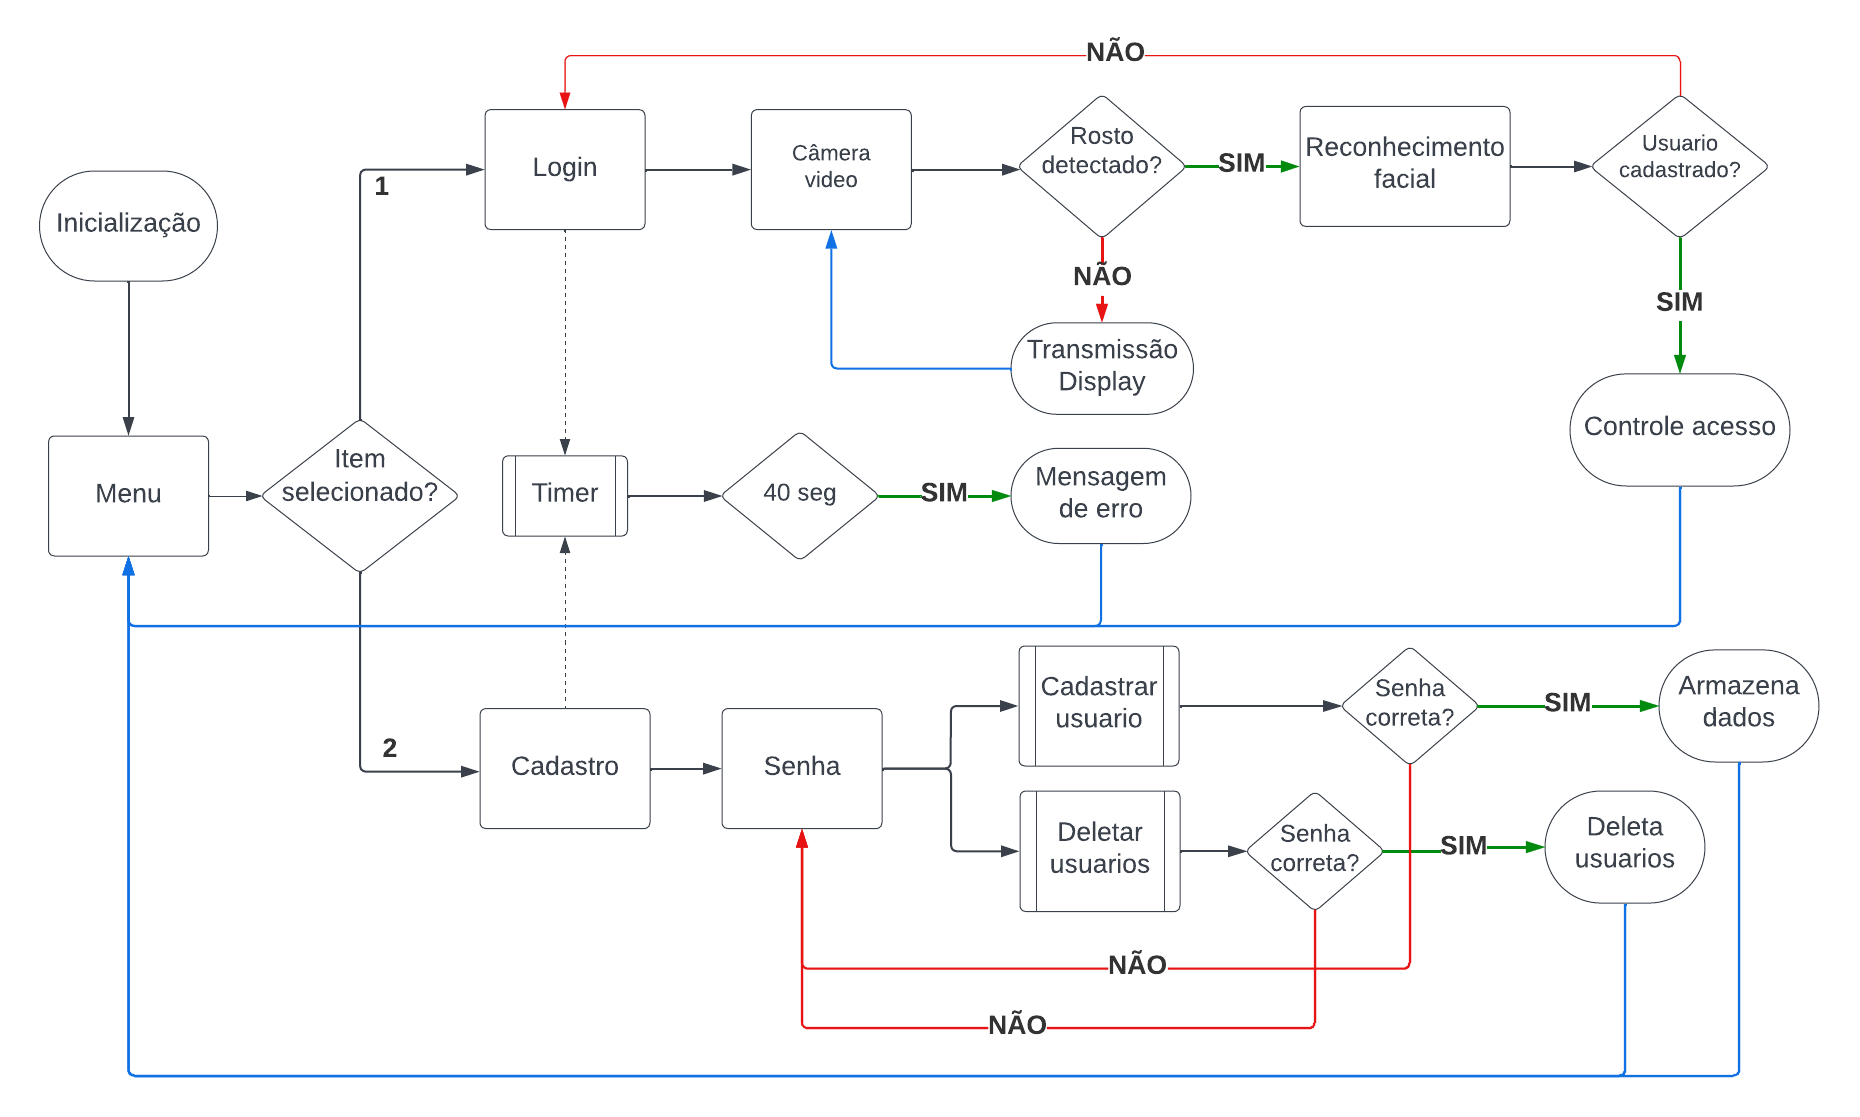
\includegraphics[scale=0.25]{figuras/fluxo_app.png}
    \fonte{}%% Fonte
    \label{fig:fluxoprog}
    \centering
\end{figure}

Para a execução desse programa, é necessário o uso de um \textit{hardware}
capaz de processá-lo. Portanto, a primeira etapa do projeto será dedicada à
construção do protótipo físico. E com o intuito de facilitar a compreensão desta
parte do projeto, foi criado o diagrama apresentado na \autoref{fig:fluxohard}.
Conforme evidenciado, o ESP32-CAM é o módulo central, encarregado do
processamento de dados e da coordenação das informações aos demais módulos.
Para melhorar a interação com os usuários, é adicionado o módulo com botões e
uma interface gráfica (display). Por fim, o módulo relé é
responsável pelo controle de acesso, podendo acionar diferentes tipos de
fechaduras elétricas.

\begin{figure}[h!]
    \centering
    \caption{Diagrama de blocos do \textit{hardware}}
    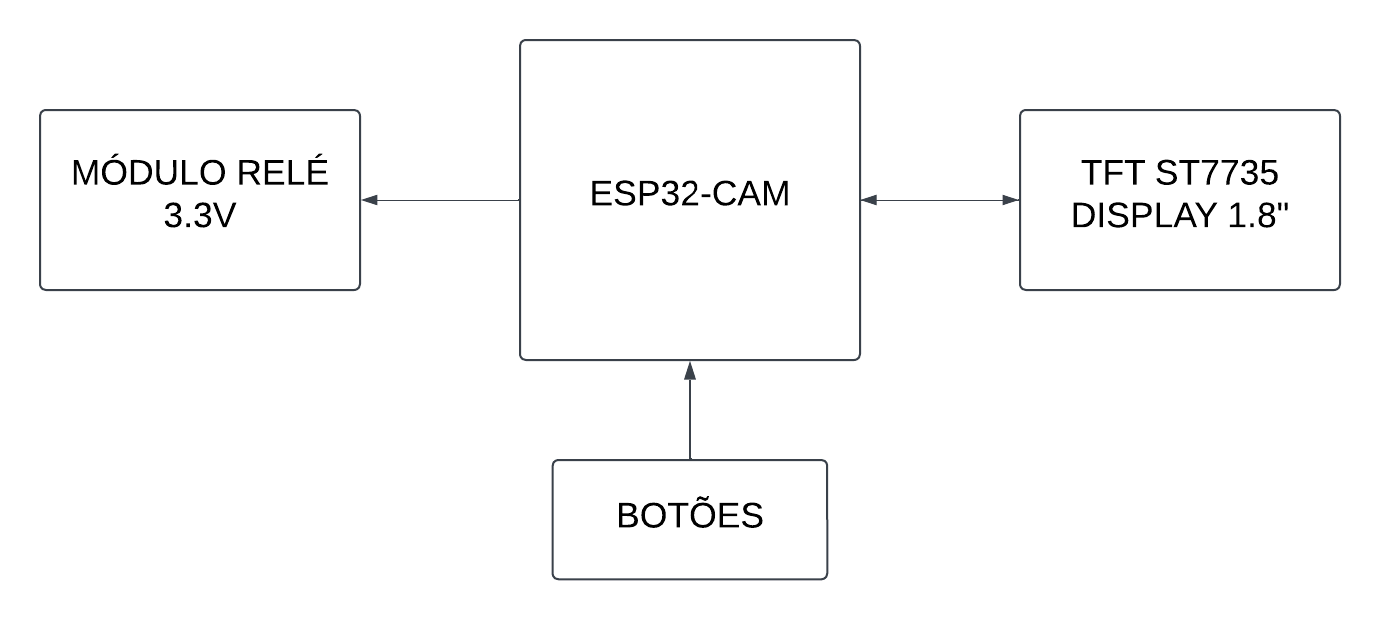
\includegraphics[scale=0.22]{figuras/diagrama_hardware.png}
    \fonte{}%% Fonte
    \label{fig:fluxohard}
    \centering
\end{figure}

Como um dos objetivos do projeto é o desenvolvimento de um protótipo de
baixo custo. A versão selecionada para essa finalidade é o ESP32-CAM,
que se destaca por integrar um \textit{chip} ESP32, uma câmera, uma
entrada para cartão SD e LED de alto brilho.

\section{Microcontrolador ESP32-CAM}\label{sec:materiais}

O ESP32-CAM (conforme ilustrado na \autoref{fig:espcam}) é um
microcontrolador de alto desempenho, desenvolvido pela empresa
\textit{Espressif Systems}® e que se destaca por sua acessibilidade.
Embora compacto, é uma escolha ideal para este projeto devido à sua
rica variedade de recursos e vantagens. Ele apresenta uma câmera
integrada à placa, um processador dual-core de 32 bits capaz de
executar tarefas em tempo real e disponibiliza 16 pinos de
Entrada/Saída (E/S).

Neste projeto, o ESP32-CAM desempenhará um papel central, sendo
responsável pelo processamento de dados, análise das informações
e controle dos demais componentes de \textit{hardware}. Isso inclui
o gerenciamento de dispositivos adicionais e a coordenação das funções
necessárias para a aplicação proposta.

\begin{figure}[h!]
    \centering
    \caption{ESP32-CAM}
    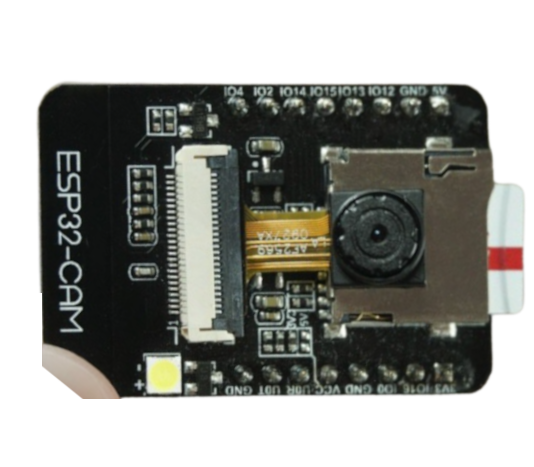
\includegraphics[scale=0.25]{figuras/esp32cam.png}
    \legend{Fonte: Adaptado de \citeonline{espcamimg}.}
    \label{fig:espcam}
    \centering
\end{figure}

\subsection{Pinos de Entrada/Saída (E/S)}\label{sec:gpio}

Os 16 pinos de Entrada/Saída (E/S) do ESP32-CAM (\autoref{fig:esp32pin})
desempenham um papel crucial na versatilidade
e funcionalidade deste microcontrolador.
Esses pinos oferecem uma interface flexível para conectar o
ESP32-CAM a uma ampla variedade de dispositivos e periféricos
externos, permitindo que ele interaja com o ambiente e execute
tarefas específicas de acordo com as necessidades do projeto.

\begin{figure}[h!]
    \centering
    \caption{GPIO disponíveis do ESP32-CAM}
    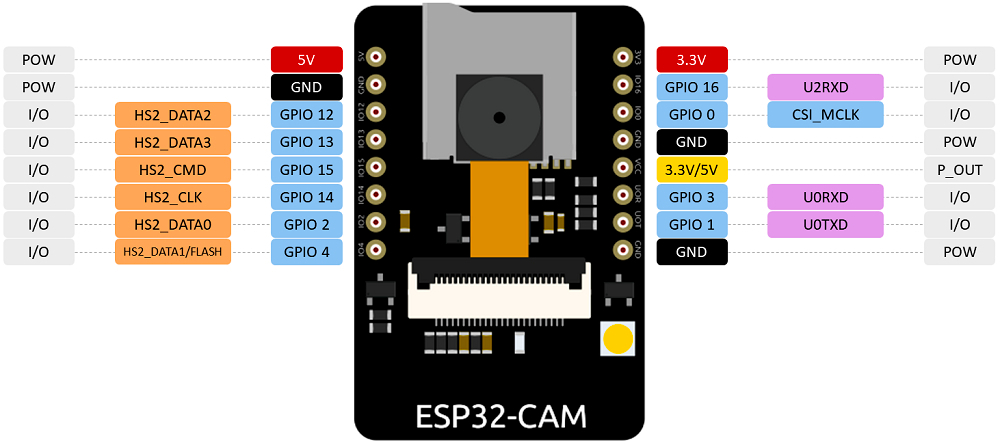
\includegraphics[scale=0.28]{figuras/esp32pin.jpg}
    \legend{Fonte: Adaptado de \citeonline{esp32pin}.}
    \label{fig:esp32pin}
    \centering
\end{figure}

Esses pinos são fundamentais para a comunicação com sensores, atuadores,
dispositivos de armazenamento, displays e muitos outros componentes
eletrônicos. Tornando o ESP32-CAM
adequado para inúmeras aplicações, desde sistemas de
segurança e monitoramento, até projetos de automação residencial..

No quadro a seguir (\autoref{quad:quadro1}), são detalhadas as funcionalidades dos 16 pinos 
de Entrada/Saída (E/S) disponíveis no ESP32-CAM. E seu entendimento, possibilita 
aos desenvolvedores a flexibilidade de personalizar e expandir suas 
aplicações de acordo com suas necessidades específicas.

\begin{tabframed}[htb]
    \caption{Portas de Entrada/Saída ESP32-CAM}
    \label{quad:quadro1}
    \begin{tabular}{|l|l|}
        \hline
        \textbf{Pinos} & \textbf{Descrição}                                                                          \\ \hline
        5V             & Pino de entrada para alimentação do circuito do ESP32.                                      \\ \hline
        3GND           & 3 pinos de aterramento, usado para referência de potencial zero                             \\ \hline
        GPIO12         & Pino de propósito geral.                                                                    \\ \hline
        GPIO13         & Pino de propósito geral.                                                                    \\ \hline
        GPIO15         & Pino de propósito geral.                                                                    \\ \hline
        GPIO14         & Pino de propósito geral.                                                                    \\ \hline
        GPIO2          & Pino de propósito geral.                                                                    \\ \hline
        GPIO4          & Pino de propósito geral e pode ser utilizado para acionar o Flash do ESP32.                 \\ \hline
        3.3V           & Pino de fornecimento de energia de 3,3V.                                                    \\ \hline
        GPIO16         & Este pino sempre fica em nível lógico alto e é utilizado para alimentar o circuto de PSRAM. \\ \hline
        GPIO0          & Pino de propósito geral, entretanto este pino é responsável pelo clock da cÂmera.           \\ \hline
        3.3V/5V        & Pode fornecer energia de 3,3V ou 5V para outros dispositivos.                               \\ \hline
        GPIO3          & Pino de entrada de dados UART (RX) para comunicação serial.                                 \\ \hline
        GPIO1          & Pino de saída de dados UART (TX) para comunicação serial.                                   \\ \hline
    \end{tabular}
    \fonte{}%% Fonte
\end{tabframed}

\section{Interface gráfica}\label{sec:interface}

O Display LCD TFT de 1.8 polegadas, com resolução de 128x160 pixels
e \textit{driver} ST7735 (\autoref{fig:tft7735}) é um componente popular 
utilizado em uma variedade de aplicações eletrônicas, devido à sua 
capacidade de fornecer uma interface visual clara e interativa. 
Esse tipo de display é frequentemente empregado em projetos que requerem 
a exibição de informações, gráficos e interação direta com o usuário.

Neste contexto, o uso deste display no projeto tem o propósito de aprimorar 
a experiência do usuário, fornecendo uma representação visual clara da 
aplicação. Além disso, sua biblioteca de fácil utilização simplifica o 
processo de desenvolvimento do projeto, tornando-o mais acessível e eficaz.

\begin{figure}[h!]
    \centering
    \caption{Display LCD TFT 1.8"}
    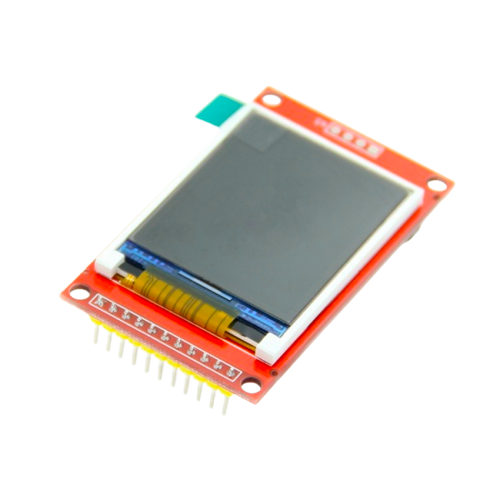
\includegraphics[scale=0.5]{figuras/tftst7735.png}
    \legend{Fonte: Adaptado de \citeonline{tft7735img}.}
    \label{fig:tft7735}
    \centering
\end{figure}

\section{Módulo de acionamento}\label{sec:acionamento}

Um módulo relé, como por exemplo, o da \autoref{fig:rele}, é um componente 
eletrônico amplamente utilizado em projetos que envolvem controle 
e automação de dispositivos elétricos. Ele desempenha 
um papel essencial ao permitir o controle de circuitos 
de alta potência por meio de sinais de baixa potência.

\begin{figure}[h!]
    \centering
    \caption{Módulo Relé}
    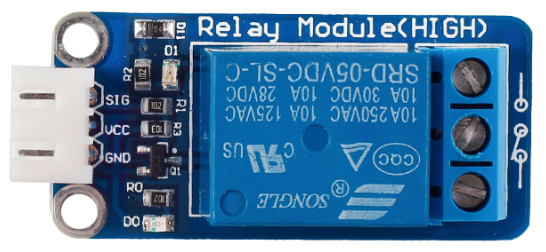
\includegraphics[scale=1]{figuras/rele.png}
    \fonte{\citeonline{releimg}}%% Fonte \legend{Fonte: Adaptado de \citeonline{releimg}.}
    \label{fig:rele}
    \centering
\end{figure}

Quando se trata de fechaduras eletrônicas, como o da \autoref{fig:fecho}, 
os módulos relé desempenham um papel crucial, facilitando o funcionamento e 
a segurança do sistema de controle de acesso. Geralmente, essas fechaduras 
incluem um mecanismo de trinco que pode ser controlado eletronicamente. 
O módulo relé é utilizado para controlar a ativação e desativação 
desse mecanismo. Quando um usuário autorizado fornece uma credencial 
válida (como uma senha, cartão RFID ou impressão digital), o sistema 
eletrônico de controle gera um sinal de baixa potência para acionar 
o módulo relé. O relé fecha seu contato, permitindo a passagem de 
energia para o mecanismo de destravamento da fechadura, liberando 
assim o acesso.

\begin{figure}[h!]
    \centering
    \caption{Fecho Elétrico}
    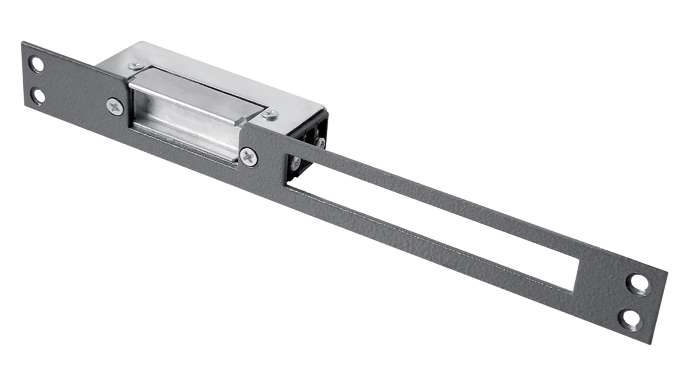
\includegraphics[scale=0.25]{figuras/fechoagl.png}
    \fonte{\citeonline{fechaduraimg}}%%\legend{Fonte: Adaptado de \citeonline{fechaduraimg}.}
    \label{fig:fecho}
    \centering
\end{figure}

\section{Desenvolvimento do software}\label{sec:software}

Para o desenvolvimento do software, foi essencial escolher uma plataforma 
de desenvolvimento capaz de programar e gravar códigos nos microcontroladores 
ESP32. Duas opções amplamente conhecidas são o Arduino IDE e o PlatformIO. 
Além disso, o desenvolvimento exigiu um estudo aprofundado das 
bibliotecas disponíveis para atender aos requisitos do projeto, 
tais como o reconhecimento facial, transmissão em tempo real de 
imagens em um display LCD, implementação de um timer e a manipulação 
dos dados de entrada e saída.

\subsection{PlatformIO}\label{sec:platformio}

A plataforma escolhida para esse projeto foi o PlatformIO, 
que é uma ferramenta indispensável para quem trabalha com dispositivos 
microcontrolados, como o ESP32. Projetado para simplificar o processo 
de desenvolvimento e programação de microcontroladores, o PlatformIO 
oferece uma ampla gama de recursos e uma abordagem unificada que 
facilita o trabalho com diferentes plataformas de hardware e 
ambientes de desenvolvimento.

Quando se trata do ESP32, o PlatformIO desempenha 
um papel crucial, permitindo que desenvolvedores e entusiastas de 
eletrônica programem e depurem suas aplicações de maneira eficiente.
O PlatformIO é projetado para funcionar com diversos editores de 
código populares, como Visual Studio Code (VSCode), Atom e CLion. 
Isso permite que os desenvolvedores escolham a IDE que melhor 
se adapte às suas preferências.

Por fim, dois outros pontos fortes do PlatformIO é que ele 
possui um gerenciador de bibliotecas embutido que facilita a 
pesquisa, instalação e atualização de bibliotecas de código-fonte 
aberto. Isso é particularmente útil para reutilizar código 
existente e acelerar o desenvolvimento. Como também sua 
simplificação no processo de compilação e carregamento de 
código para o hardware de destino. 

\subsection{Bibliotecas}\label{sec:formatacaoTexto}

Para identificação de rostos e reconhecimento facial, foram utilizados 
os recursos disponiveis da biblioteca ESP-DL.

O ESP-DL é uma biblioteca de alto desempenho dedicada ao ESP32, ESP32-S2,
ESP32-S3 e ESP32-C3, projetada para recursos de aprendizagem profunda.

O \citeonline{espdl} disponibiliza APIs para tarefas como inferência 
de redes neurais (NN), processamento de imagens, operações matemáticas 
e inclui alguns modelos de aprendizado profundo. Com essa biblioteca, 
os desenvolvedores podem aproveitar os SoCs (System-on-Chip) da 
\textit{Espressif} de maneira simples e ágil para a implementação 
de uma ampla variedade de aplicações.




\begin{figure}[h!]
    \centering
    \caption{Diagrama elétrico do protótipo}
    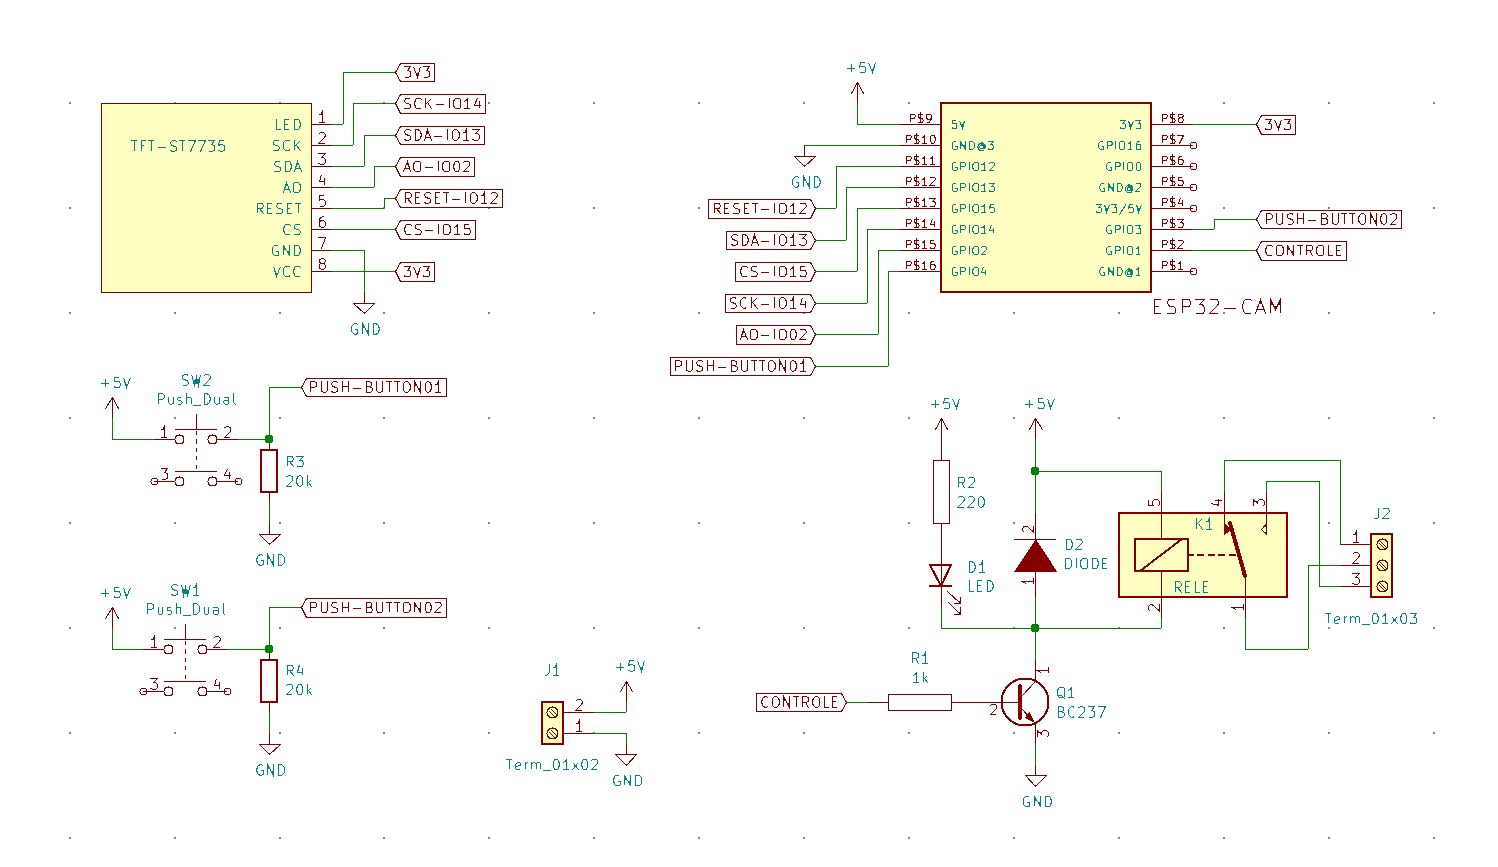
\includegraphics[scale=0.3]{figuras/circuito_completo.png}
    \fonte{}%% Fonte
    \label{fig:circuito}
    \centering
\end{figure}

\begin{figure}[h!]
    \centering
    \caption{Diagrama elétrico do Display TFT}
    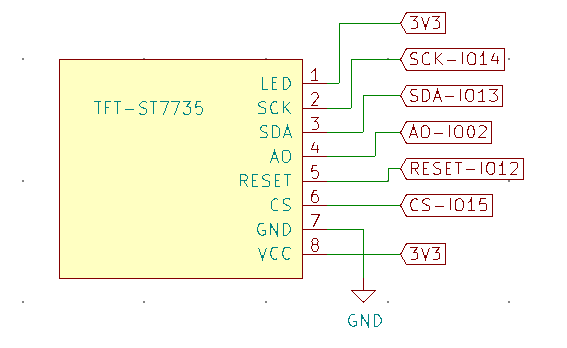
\includegraphics[scale=0.4]{figuras/modulo_tft.png}
    \fonte{}%% Fonte
    \label{fig:diagramatft}
    \centering
\end{figure}

\begin{figure}[h!]
    \centering
    \caption{Diagrama elétrico do ESP32-CAM}
    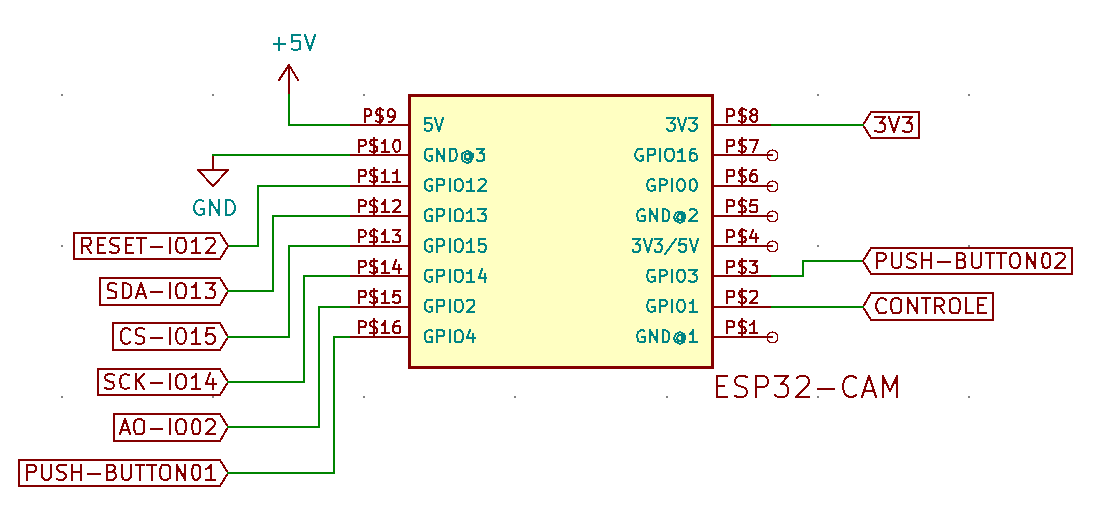
\includegraphics[scale=0.35]{figuras/modulo_esp.png}
    \fonte{}%% Fonte
    \label{fig:diagramaesp}
    \centering
\end{figure}

\begin{figure}[h!]
    \centering
    \caption{Diagrama elétrico dos botões}
    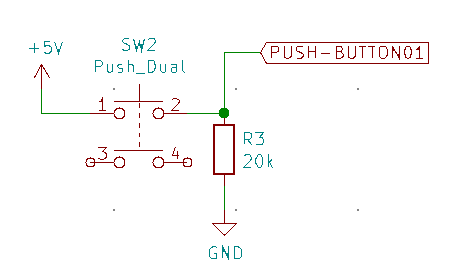
\includegraphics[scale=0.4]{figuras/modulo-push-button.png}
    \fonte{}%% Fonte
    \label{fig:diagramabotoes}
    \centering
\end{figure}

\begin{figure}[h!]
    \centering
    \caption{Diagrama elétrico acionamento relé}
    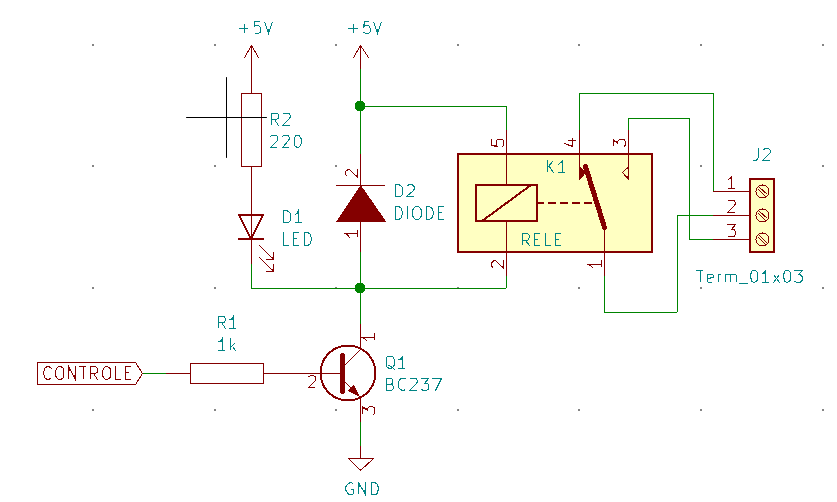
\includegraphics[scale=0.4]{figuras/modulo_rele_esquema.png}
    \fonte{}%% Fonte
    \label{fig:diagramarele}
    \centering
\end{figure}

\begin{figure}[h!]
    \centering
    \caption{Telas de inicialização}
    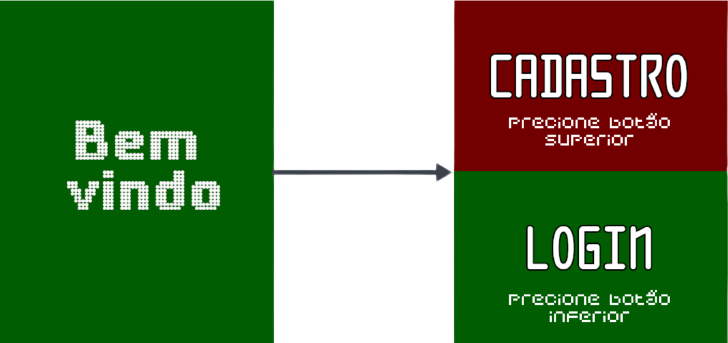
\includegraphics[scale=0.3]{figuras/fluxo_inicial.png}
    \fonte{}%% Fonte
    \label{fig:fluxoinicial}
    \centering
\end{figure}

\begin{figure}[h!]
    \centering
    \caption{Telas login}
    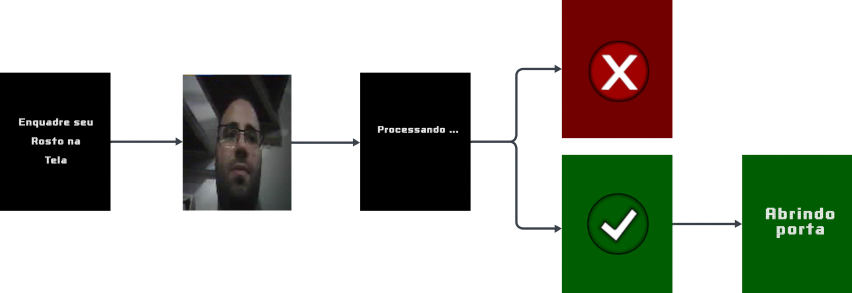
\includegraphics[scale=2.2]{figuras/fluxo_login.png}
    \fonte{}%% Fonte
    \label{fig:fluxologin}
    \centering
\end{figure}

\begin{figure}[h!]
    \centering
    \caption{Telas cadastro}
    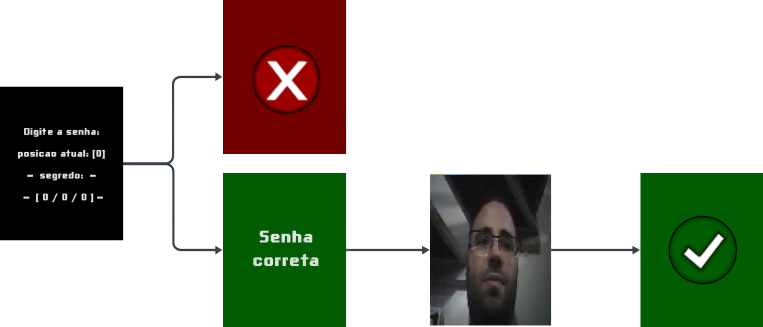
\includegraphics[scale=2.5]{figuras/fluxo_cadastro.png}
    \fonte{}%% Fonte
    \label{fig:fluxocadastro}
    \centering
\end{figure}

\begin{figure}[h!]
    \centering
    \caption{Telas deletar usuario}
    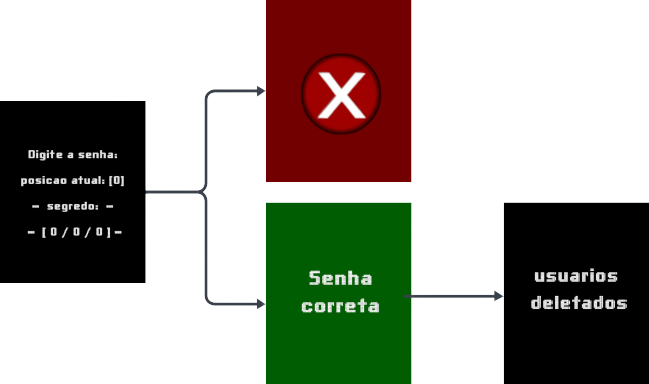
\includegraphics[scale=2.5]{figuras/fluxo_deletar_usuario.png}
    \fonte{}%% Fonte
    \label{fig:fluxosenha}
    \centering
\end{figure}

\begin{figure}[h!]
    \centering
    \caption{Projeto da placa de circuito impresso do protótipo}
    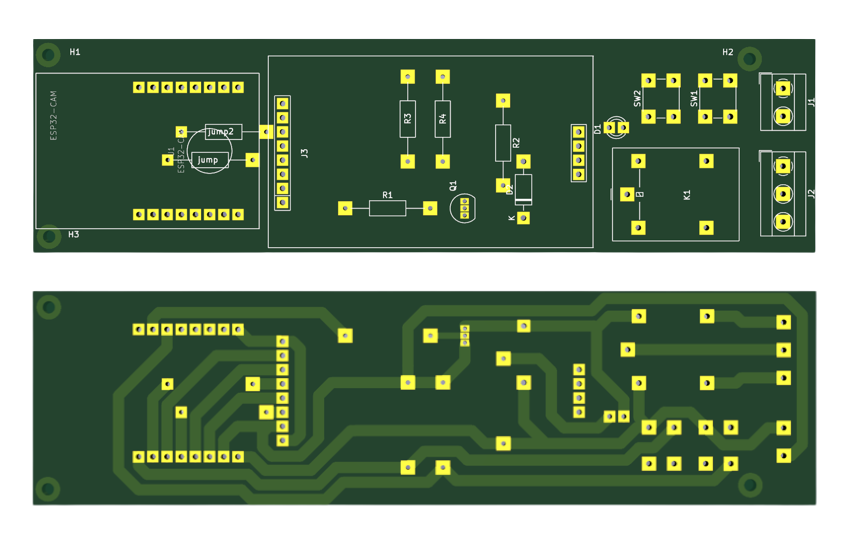
\includegraphics[scale=0.35]{figuras/placa_pcb.png}
    \fonte{}%% Fonte
    \label{fig:placapcb}
    \centering
\end{figure}

\begin{figure}[h!]
    \centering
    \caption{Placa manufaturada}
    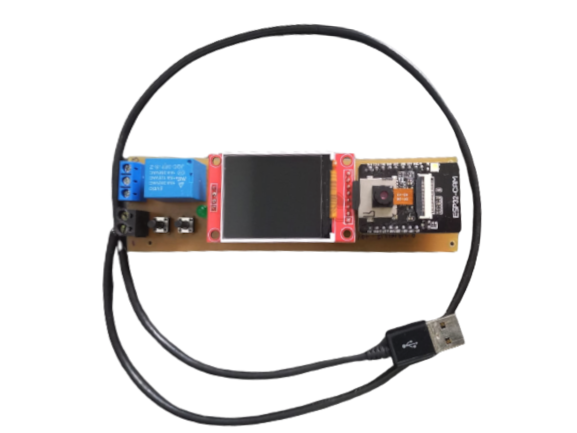
\includegraphics[scale=0.45]{figuras/placa_montada.png}
    \fonte{}%% Fonte
    \label{fig:placamanufaturada}
    \centering
\end{figure}